\section{Iteration 3}
TODO Einleitung
Dabei sind folgenden Rückmeldungen entstanden:
\begin{itemize}
    \item Die für Desktops optimiert Benutzerschnittelle entspricht den Vorstellungen und wirkt intuitiv.
    \item Da vom Auftraggeber keine echten \ac{THD} Werte zur Verfügung gestellt werden können,
    können diese weggelassen werden.
    \item Die Applikation soll unm die in der Aufgabenstellung (Anhang \ref{anhang:aufgabenstellung}) beschrieben Anforderung:
    ``Eine benutzerdefinierte Zeitspanne der Messwerte mittels vorgegebener
    Labels beschriften. Bsp.: («Backofen war von 09:31 – 10:15 aktiv»)`` soll implementiert werden.
    \item Die Übertragung der Messdaten mittels \ac{MQTT} soll,
     wie bereits in der Aufgabenstellung (Anhang \ref{anhang:aufgabenstellung}) verlangt, mit \ac{TLS} verschlüsselt werden.
\end{itemize}

\subsection{TLS Verschlüsselung}

\subsection{Benutzerschnittstelle}
% \subsection{Labeling}
% - Labeling:
% Labels graphisch darstellen
% Labels mittels UI hinzufügen

\subsection{Verifikation}

Um die korrekte Funktionalität der neu implementierten Anforderungen zu verifizieren, wurden
zwei neue End to End Tests implementiert. Diese verifizieren zum einen die Funktionalität der
Labelerstellung und zum anderen, ob die \ac{TLS} Verschlüsselung funktioniert (Abbildung \ref{fig:test-iteration-3}).

\begin{figure}[h]
    \centering
    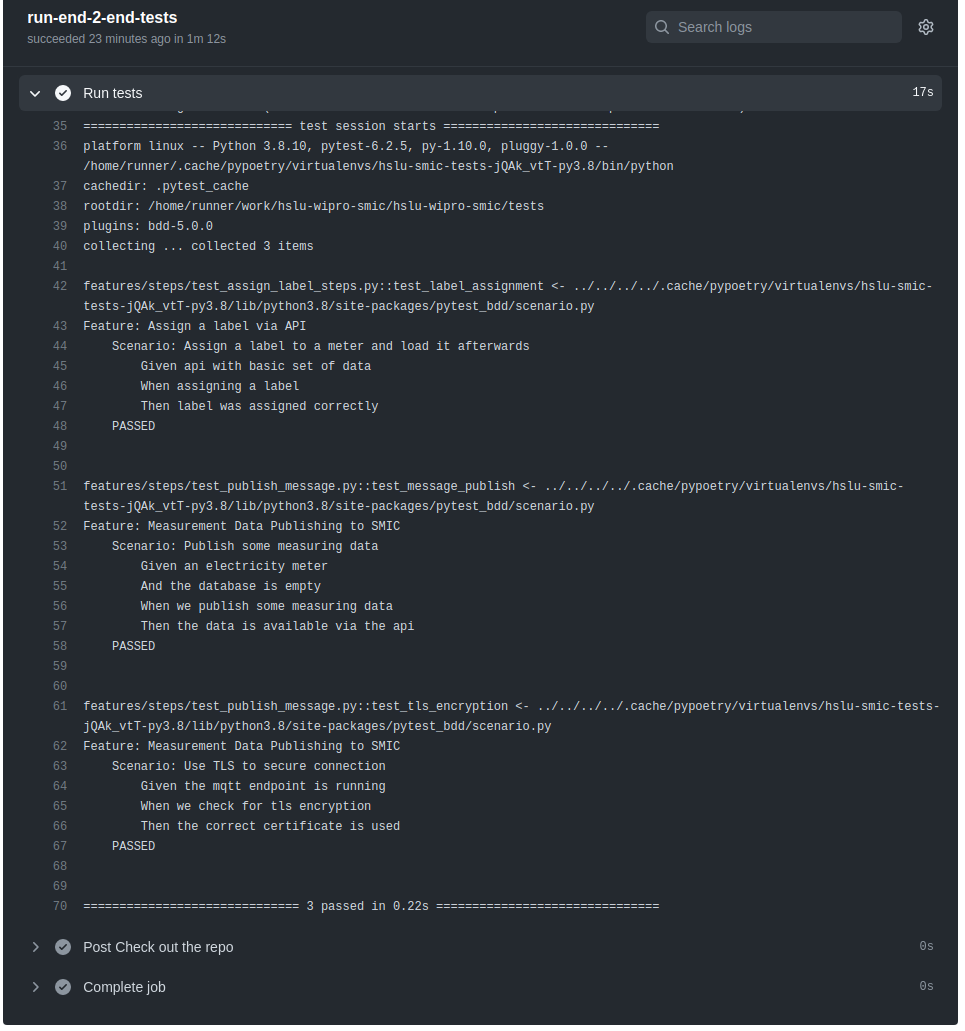
\includegraphics[width=1.0\textwidth]{gfx/testlog-iteration-2}
    \caption{
        Erweiterung der Tests um das Assignment der Labels und Testen der \ac{TLS} Verschlüsselung \parencite{randombenj_testlog_it_2_2021}.
    }
    \label{fig:test-iteration-3}
\end{figure}

\subsection{Schwierigkeiten}
TLS..